% !TEX root=../main.tex
\documentclass[beamer]{standalone}
\begin{document}
% ==============================================================
% Method : Gradient Descenet Explanations - 7 (Original Adam vs Uniform Adam)
% ============================================================== 
\begin{frame}{Method}
\framesubtitle{Momentum and Variance}

\begin{columns}[T] % align columns
\begin{column}{.45\textwidth}
\begin{algorithm}[H]
    \begin{algorithmic}[1]
        \WHILE{$x$ not converged do}
            \STATE $g \leftarrow (I + \lambda L)^{-1} \diffp{\Phi}{x}$
            \STATE $m_{1} \leftarrow \beta_{1} m_{1} + (1-\beta_{1})g$
            \STATE $m_{2} \leftarrow \beta_{1} m_{2} + (1-\beta_{1})g^2$
            \STATE $u \leftarrow u-\frac{\eta}{(1-\beta_{1}^{k}) \sqrt{\frac{\left\lVert m_{2} \right\rVert_{\infty}}{1-\beta_{2}^{k}}}}$
        \ENDWHILE
        \STATE where $x(u)=(I+\lambda L)^{-1}u$
        \end{algorithmic}
    \caption{UniformAdam}
    \label{alg:seq}
    \end{algorithm}
\end{column}
\begin{column}{0.45\textwidth}
    \begin{figure}
        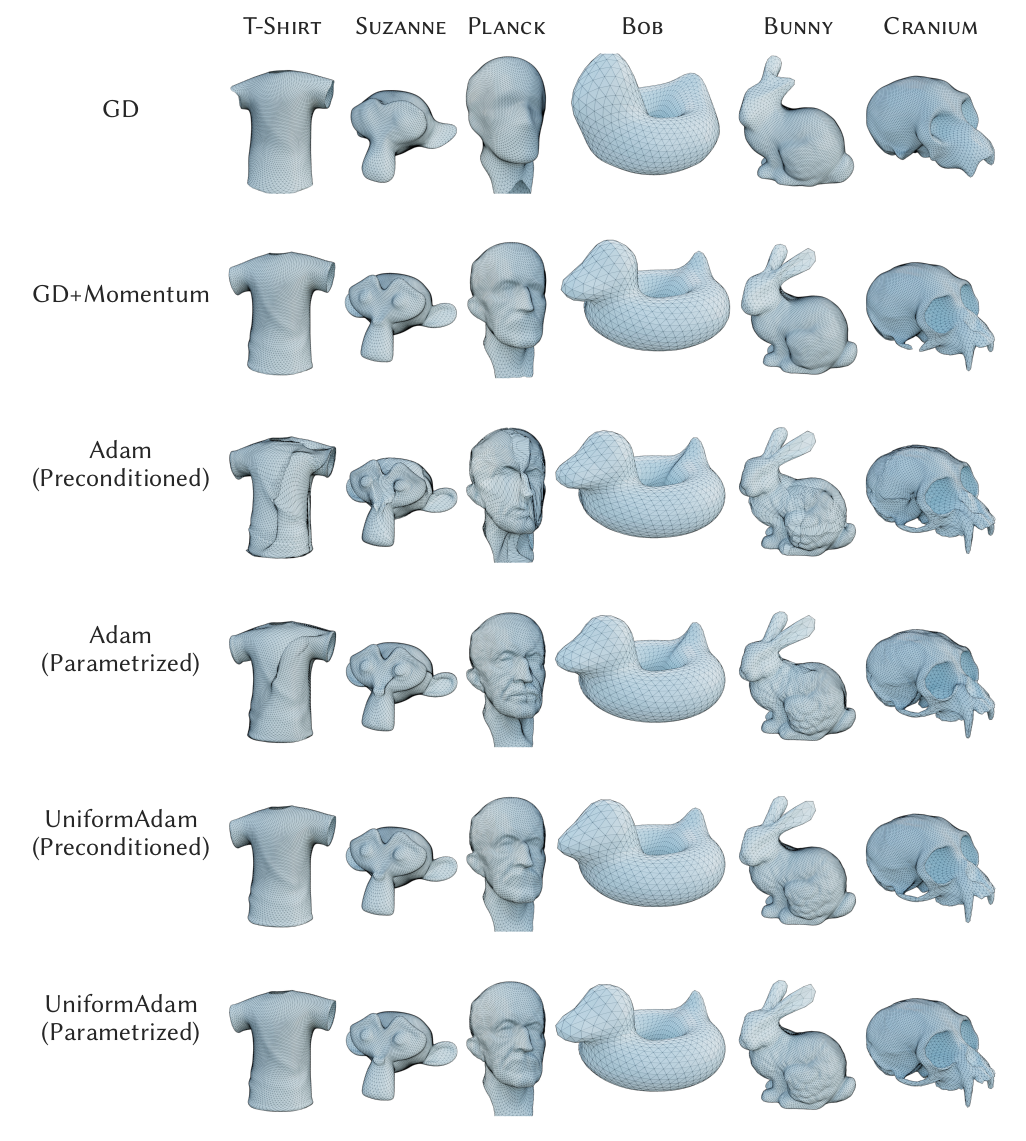
\includegraphics[width=\textwidth]{figures/method3-figure-1.png}
    \end{figure}
\end{column}
\end{columns}

% note %
\note[item] {
    Until now, I have explained the main idea of this paper.

    This is final form their implementation of Adam.

    The authors said that they discovered that aggresive steps disturb the smoothness of result.
    So, they modify it to a more uniform adaptation, and the picture of rightside is the comparison.
}
\end{frame}

% ==============================================================
% Method : Gradient Descenet Explanations - other details (implementation, )
% ============================================================== 
\begin{frame}{Method}
\framesubtitle{Remeshing}
\begin{itemize}
    \item Remeshing
    \begin{enumerate}
        \item remeshing is the technique that rebalance the energy of mesh
        \item In this paper, the authors adapted isotropic remeshing (Bostch and Kobbelt [2004])
        \item remeshing at manually specified timesteps
    \end{enumerate}
    \begin{figure}
        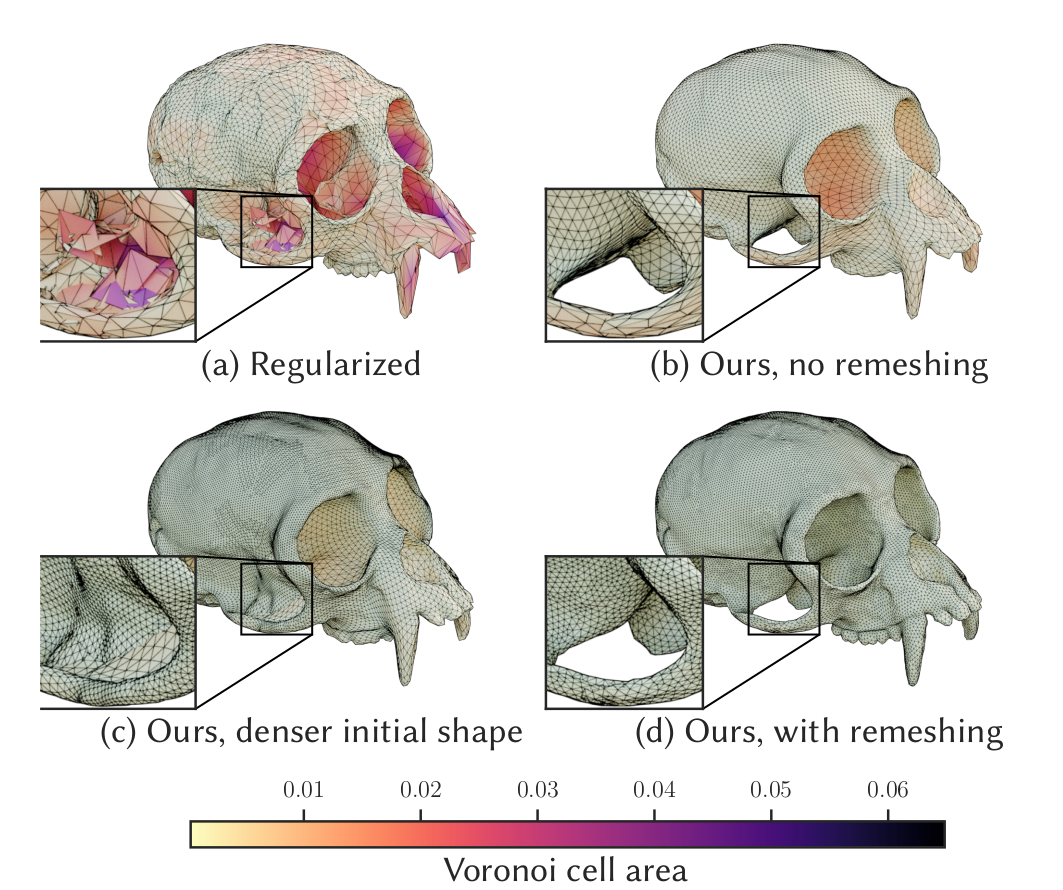
\includegraphics[width=0.5\textwidth]{figures/method3-figure-2.png}
    \end{figure}
\end{itemize}

% note %
\note[item] {
    And lastly, they use remeshing technique to solve the mesh energy balancing and resolution problem.
    
    Remeshing is the technique that rebalance the energy of mesh, by resampling vertices and modifying edge length.
    There are several remeshing technique, in this paper they adapt isotropic remeshing from Bostch and Kobbelt, the original paper title is "A Remeshing Approach to Multiresolution Modeling"
} 

\end{frame}
\end{document}